\documentclass[journal,12pt,twocolumn]{IEEEtran}

\usepackage{setspace}
\usepackage{gensymb}

\singlespacing


\usepackage[cmex10]{amsmath}

\usepackage{amsthm}

\usepackage{mathrsfs}
\usepackage{txfonts}
\usepackage{stfloats}
\usepackage{bm}
\usepackage{cite}
\usepackage{cases}
\usepackage{subfig}

\usepackage{longtable}
\usepackage{multirow}

\usepackage{enumitem}
\usepackage{mathtools}
\usepackage{steinmetz}
\usepackage{tikz}
\usepackage{circuitikz}
\usepackage{verbatim}
\usepackage{tfrupee}
\usepackage[breaklinks=true]{hyperref}
\usepackage{graphicx}
\usepackage{tkz-euclide}

\usetikzlibrary{calc,math}
\usepackage{listings}
\usepackage{color}                                            %%
\usepackage{array}                                            %%
\usepackage{longtable}                                        %%
\usepackage{calc}                                             %%
\usepackage{multirow}                                         %%
\usepackage{hhline}                                           %%
\usepackage{ifthen}                                           %%
\usepackage{lscape}     
\usepackage{multicol}
\usepackage{chngcntr}

\DeclareMathOperator*{\Res}{Res}

\renewcommand\thesection{\arabic{section}}
\renewcommand\thesubsection{\thesection.\arabic{subsection}}
\renewcommand\thesubsubsection{\thesubsection.\arabic{subsubsection}}

\renewcommand\thesectiondis{\arabic{section}}
\renewcommand\thesubsectiondis{\thesectiondis.\arabic{subsection}}
\renewcommand\thesubsubsectiondis{\thesubsectiondis.\arabic{subsubsection}}


\hyphenation{op-tical net-works semi-conduc-tor}
\def\inputGnumericTable{}                                 %%

\lstset{
	%language=C,
	frame=single, 
	breaklines=true,
	columns=fullflexible
}
\begin{document}
	
	
	\newtheorem{theorem}{Theorem}[section]
	\newtheorem{problem}{Problem}
	\newtheorem{proposition}{Proposition}[section]
	\newtheorem{lemma}{Lemma}[section]
	\newtheorem{corollary}[theorem]{Corollary}
	\newtheorem{example}{Example}[section]
	\newtheorem{definition}[problem]{Definition}
	
	\newcommand{\BEQA}{\begin{eqnarray}}
		\newcommand{\EEQA}{\end{eqnarray}}
	\newcommand{\define}{\stackrel{\triangle}{=}}
	\bibliographystyle{IEEEtran}
	\providecommand{\mbf}{\mathbf}
	\providecommand{\pr}[1]{\ensuremath{\Pr\left(#1\right)}}
	\providecommand{\qfunc}[1]{\ensuremath{Q\left(#1\right)}}
	\providecommand{\sbrak}[1]{\ensuremath{{}\left[#1\right]}}
	\providecommand{\lsbrak}[1]{\ensuremath{{}\left[#1\right.}}
	\providecommand{\rsbrak}[1]{\ensuremath{{}\left.#1\right]}}
	\providecommand{\brak}[1]{\ensuremath{\left(#1\right)}}
	\providecommand{\lbrak}[1]{\ensuremath{\left(#1\right.}}
	\providecommand{\rbrak}[1]{\ensuremath{\left.#1\right)}}
	\providecommand{\cbrak}[1]{\ensuremath{\left\{#1\right\}}}
	\providecommand{\lcbrak}[1]{\ensuremath{\left\{#1\right.}}
	\providecommand{\rcbrak}[1]{\ensuremath{\left.#1\right\}}}
	\theoremstyle{remark}
	\newtheorem{rem}{Remark}
	\newcommand{\sgn}{\mathop{\mathrm{sgn}}}
	\providecommand{\abs}[1]{\left\vert#1\right\vert}
	\providecommand{\res}[1]{\Res\displaylimits_{#1}} 
	\providecommand{\norm}[1]{\left\lVert#1\right\rVert}
	%\providecommand{\norm}[1]{\lVert#1\rVert}
	\providecommand{\mtx}[1]{\mathbf{#1}}
	\providecommand{\mean}[1]{E\left[ #1 \right]}
	\providecommand{\fourier}{\overset{\mathcal{F}}{ \rightleftharpoons}}
	%\providecommand{\hilbert}{\overset{\mathcal{H}}{ \rightleftharpoons}}
	\providecommand{\system}{\overset{\mathcal{H}}{ \longleftrightarrow}}
	%\newcommand{\solution}[2]{\textbf{Solution:}{#1}}
	\newcommand{\solution}{\noindent \textbf{Solution: }}
	\newcommand{\cosec}{\,\text{cosec}\,}
	\providecommand{\dec}[2]{\ensuremath{\overset{#1}{\underset{#2}{\gtrless}}}}
	\newcommand{\myvec}[1]{\ensuremath{\begin{pmatrix}#1\end{pmatrix}}}
	\newcommand{\mydet}[1]{\ensuremath{\begin{vmatrix}#1\end{vmatrix}}}
	\numberwithin{equation}{subsection}
	\makeatletter
	\@addtoreset{figure}{problem}
	\makeatother
	\let\StandardTheFigure\thefigure
	\let\vec\mathbf
	\renewcommand{\thefigure}{\theproblem}
	\def\putbox#1#2#3{\makebox[0in][l]{\makebox[#1][l]{}\raisebox{\baselineskip}[0in][0in]{\raisebox{#2}[0in][0in]{#3}}}}
	\def\rightbox#1{\makebox[0in][r]{#1}}
	\def\centbox#1{\makebox[0in]{#1}}
	\def\topbox#1{\raisebox{-\baselineskip}[0in][0in]{#1}}
	\def\midbox#1{\raisebox{-0.5\baselineskip}[0in][0in]{#1}}
	\vspace{3cm}
	
	
	
	\title{EE5609 Assignment 6}
	\author{Vimal K B \\Roll No - AI20MTECH12001}
	
	\maketitle
	\newpage
	%\tableofcontents
	\bigskip
	
	\renewcommand{\thefigure}{\theenumi}
	\renewcommand{\thetable}{\theenumi}
	
	\begin{abstract}
		This assignment involves finding the equation for two tangents to the curve. In the first cases the tangent is parallel to the given line. In the second case, the tangent is perpendicular to the given line.
	\end{abstract}
	
The python solution code for this problem can be downloaded from

\begin{lstlisting}
	https://github.com/vimalkb007/EE5609/tree/master/Assignment_6/codes
\end{lstlisting}
	
	\section{Problem Statement}
	Find the equation of the tangent line to the curve $y = x^2-2x+7$
	
	\begin{enumerate}
		\item  parallel to the line $\myvec{2 & -1}\vec{x}= -9$ 
		\item  perpendicular to the line $\myvec{-15 & 5}\vec{x} = 13$.
	\end{enumerate}
	 
	
	\section{Solution}
		Given equation 
		\begin{align} \label{eq:fact1}
			y = x^2-2x+7
		\end{align}
	
		The equation \eqref{eq:fact1} can be written as,
		\begin{align}
			x^2-2x-y+7 = 0
		\end{align}
		Comparing it with standard equation,
		\begin{align}
			ax^2+2bxy+cy^2+2dx+2ey+f = 0
		\end{align}
		$\therefore$ a = 1, b = 0, c = 0, d = -1, e = $\frac{-1}{2}$, f = 7.
		\begin{align}
			\therefore \vec{V} = \myvec{a&b\\b&c} = \myvec{1&0\\0&0}
		\end{align} 
		\begin{align}
			\therefore\vec{u} = \myvec{d\\e} = \myvec{-1\\\frac{-1}{2}}\label{eq:eq1}
		\end{align}
		\begin{align}
			\mbox{ Now,} \mydet{V} = \mydet{1&0\\0&0} = 0
		\end{align}
		$\implies$ that the curve is a parabola. Now, finding the eigen values corresponding to the $\vec{V}$,
		\begin{align}
			\mydet{\vec{V}-\lambda\vec{I}} = 0
		\end{align}
		\begin{align}
			\mydet{1-\lambda&0\\0&-\lambda} = 0
		\end{align}
		\begin{align}
			\implies \lambda = 0,1.
		\end{align}
		Calculating the eigenvectors corresponding to $\lambda = 0,1$ respectively,
		\begin{align}
			\vec{V}\vec{x} = \lambda\vec{x}
		\end{align}
		\begin{align}
			\myvec{1&0\\0&0}\vec{x} = 0 \implies \vec{p_1} = \myvec{0\\1}
		\end{align}
		\begin{align}
			\myvec{0&0\\0&-1}\vec{x} = \vec{x} \implies \vec{p_2} = \myvec{1\\0}
		\end{align}
		Now by eigen decomposition on $\vec{V}$,
		\begin{align}
			\vec{V} = \vec{PDP^T}
			\label{eq:eq2}
		\end{align}
		\begin{align}
			\mbox{where,} \vec{P} = \myvec{\vec{p_1} \vec{p_2}} = \myvec{0&1\\1&0}
		\end{align}
		\begin{align}
			\vec{D} = \myvec{\lambda_1&0\\0&\lambda_2} = \myvec{0&0\\0&1}
		\end{align}
		Hence equation \eqref{eq:eq1} becomes,
		\begin{align}
			\vec{V} = \myvec{0&1\\1&0}\myvec{0&0\\0&1}\myvec{0&1\\1&0}
		\end{align}
		\begin{align}
			\vec{V} = \myvec{1&0\\0&0}
		\end{align}
	
	\begin{enumerate}
		\item
							The given parallel line equation is
		\begin{align} 
			\myvec{2 & -1}\vec{x}= -9 \\
			\implies 2x - y + 9 = 0 \label{eq:fact2}
		\end{align}
		Now the tangent to parabola is parallel to the line equation \eqref{eq:fact2}, the general straight line equation is of the form
		\begin{align}
			ax + by + c = 0
		\end{align}
		The normal vector ($\vec{n}$) and direction ($\vec{m}$) are given by,
		\begin{align} 
			\vec{n} = \myvec{a\\b} \label{eq:eq3}\\
			\vec{m} = \myvec{b\\-a} \label{eq:eq4}
		\end{align}
		Comparing \eqref{eq:fact2}, \eqref{eq:eq2}, \eqref{eq:eq3}, the direction vectors ($\vec{m}$) and normal ($\vec{n}$)  vectors are,
		\begin{align}
			\vec{m} = \myvec{-1\\-2}\\
			\vec{n} = \myvec{2\\-1}\label{eq:eq5}
		\end{align} 
		Now, the equation for the point of contact for the parabola is given as,
		\begin{align}
			\myvec{\vec{u}^T+\kappa\vec{n}^T\\\vec{V}}\vec{q} = \myvec{-f\\\kappa\vec{n}-\vec{u}}\label{eq:eq6}\\
			\mbox{where, } \kappa = \frac{\vec{p_1}^T\vec{u}}{\vec{p_1}^T\vec{n}} = \frac{1}{2} \label{eq:eq7}
		\end{align}
		Hence substituting the values of \eqref{eq:eq1}, \eqref{eq:eq5}, \eqref{eq:eq2}, \eqref{eq:eq7} in equation \eqref{eq:eq6} we get,
		\begin{align}
			\myvec{0&-1\\1&0\\0&0}\vec{q} = \myvec{-7\\2\\0}
			\label{eq:eq8}
		\end{align}
		Solving for $\vec{q}$ by removing the zero row and representing \eqref{eq:eq8} as augmented matrix and then converting the matrix to echelon form,
		\begin{align}
			\implies \myvec{0&-1&-7\\1&0&2} \xleftrightarrow[]{R_1\xleftrightarrow[]{}R_2} \myvec{1&0&2\\0&-1&-7}
		\end{align}
		\begin{align}
			\xleftrightarrow[]{R_2\leftarrow  -R_2} \myvec{1&0&2\\0&1&7}
			\label{eq:eq9}
		\end{align}
		Hence from equation \eqref{eq:eq9} it can be concluded that the point of contact is,
		\begin{align}
			\vec{q} = \myvec{2\\7}
		\end{align}
		Now $\vec{q}$ is a point on the tangent. Hence, the equation of the
		line can be expressed as
		\begin{align}
			\vec{n}^T\vec{x} = c
			\label{eq:eq10}
		\end{align}
		where c is,
		\begin{align}
			c = \vec{n}^T\vec{q} = \myvec{2&-1}\myvec{2\\7} = -3 
			\label{eq:eq11}
		\end{align}
		Hence equation of tangent to the curve \eqref{eq:fact1} parallel to \eqref{eq:fact2} is given by substituting the value of c and $\vec{n}$ from equation \eqref{eq:eq11} and \eqref{eq:eq5} respectively to the equation \eqref{eq:eq10},
		\begin{align}
			\implies\myvec{2&-1}\vec{x} = -3 
		\end{align}
		Figure \ref{eq:fig1} verifies that the $\myvec{2&-1}\vec{x} = -3$ is a tangent to parabola  $y = x^2-2x+7$
		\begin{figure}[ht!]
			\centering
			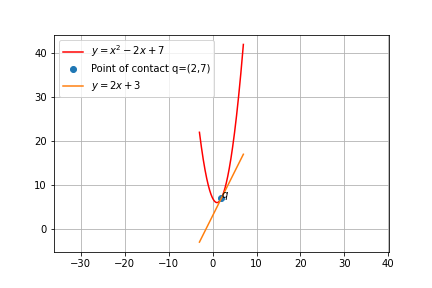
\includegraphics[width=\columnwidth]{./codes/parallelLineTangent.png}
			\caption{Tangent to parabola $y = x^2-2x+7$}
			\label{eq:fig1}
		\end{figure}
	
	\item
						The given perpendicular line equation is
	\begin{align} 
		\myvec{-15 & 5}\vec{x}= 13 \\
		\implies -15x + 5y - 13 = 0 \label{eq:fact3}
	\end{align}
	Now the tangent to parabola is perpendicular to the line equation \eqref{eq:fact3}, the general straight line equation is of the form
	\begin{align}
		ax + by + c = 0
	\end{align}
	Therefore, if we find the line that is parallel to the line \eqref{eq:fact3}, it will be parallel to the tangent itself. For the given line the normal vector ($\vec{n}$) and direction ($\vec{m}$) are given by,
	\begin{align} 
		\vec{n} = \myvec{a\\b} \label{eq:eq12}\\
		\vec{m} = \myvec{b\\-a} \label{eq:eq13}
	\end{align}
	Comparing \eqref{eq:fact3}, \eqref{eq:eq12}, \eqref{eq:eq13}, the direction vectors ($\vec{m}$) and normal ($\vec{n}$)  vectors are,
	\begin{align}
		\vec{m} = \myvec{5\\15}\\
		\vec{n} = \myvec{-15\\5}\label{eq:eq14}
	\end{align} 

	The parallel line for this vector will have the normal vector ($\vec{n_1}$) and direction ($\vec{m_1}$) are given by
	
		\begin{align}
		\vec{m_1} = \myvec{15\\-5}\\
		\vec{n_1} = \myvec{5\\15}\label{eq:eq15}
	\end{align} 
	
	Now, the equation for the point of contact for the parabola is given as,
	\begin{align}
		\myvec{\vec{u}^T+\kappa\vec{n_1}^T\\\vec{V}}\vec{q} = \myvec{-f\\\kappa\vec{n_1}-\vec{u}}\label{eq:eq16}\\
		\mbox{where, } \kappa = \frac{\vec{p_1}^T\vec{u}}{\vec{p_1}^T\vec{n_1}} = \frac{-1}{30} \label{eq:eq17}
	\end{align}
	Hence substituting the values of \eqref{eq:eq1}, \eqref{eq:eq15}, \eqref{eq:eq2}, \eqref{eq:eq17} in equation \eqref{eq:eq16} we get,
	\begin{align}
		\myvec{\frac{-7}{6}&-1\\1&0\\0&0}\vec{q} = \myvec{-7\\\frac{5}{6}\\0}
		\label{eq:eq18}
	\end{align}
	Solving for $\vec{q}$ by removing the zero row and representing \eqref{eq:eq18} as augmented matrix and then converting the matrix to echelon form,
	\begin{align}
		\implies \myvec{\frac{-7}{6}&-1&-7\\1&0&\frac{5}{6}} \xleftrightarrow[]{R_1\xleftrightarrow[]{}R_2} \myvec{1&0&\frac{5}{6}\\\frac{-7}{6}&-1&-7}
	\end{align}
	\begin{align}
		\xleftrightarrow[]{R_2\leftarrow R_2-\brak{\frac{7}{6}}R_1} \myvec{1&0&\frac{5}{6}\\0&-1&\frac{-217}{36}} \\
		\xleftrightarrow[]{R_2\leftarrow  -R_2} \myvec{1&0&\frac{5}{6}\\0&1&\frac{217}{36}}
		\label{eq:eq19}
	\end{align}
	Hence from equation \eqref{eq:eq19} it can be concluded that the point of contact is,
	\begin{align}
		\vec{q} = \myvec{\frac{5}{6}\\\frac{217}{36}}
	\end{align}
	Now $\vec{q}$ is a point on the tangent. Hence, the equation of the
	line can be expressed as
	\begin{align}
		\vec{n_1}^T\vec{x} = c
		\label{eq:eq20}
	\end{align}
	where c is,
	\begin{align}
		c = \vec{n_1}^T\vec{q} = \myvec{5&15}\myvec{\frac{5}{6}\\\frac{217}{36}} = \frac{3405}{36} 
		\label{eq:eq21}
	\end{align}
	Hence equation of tangent to the curve \eqref{eq:fact1} parallel to \eqref{eq:fact3} is given by substituting the value of c and $\vec{n_1}$ from equation \eqref{eq:eq21} and \eqref{eq:eq15} respectively to the equation \eqref{eq:eq20},
	\begin{align}
		\implies\myvec{5&15}\vec{x} = \frac{3405}{36} 
	\end{align}
	Figure \ref{eq:fig2} verifies that the $\myvec{5&15}\vec{x} = \frac{3405}{36}$ is a tangent to parabola  $y = x^2-2x+7$
	\begin{figure}[ht!]
		\centering
		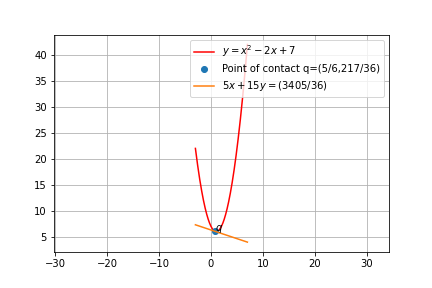
\includegraphics[width=\columnwidth]{./codes/perpendicularLineTangent.png}
		\caption{Tangent to parabola $y = x^2-2x+7$}
		\label{eq:fig2}
	\end{figure}

	\end{enumerate}
		
	
\end{document}